\listfiles
\documentclass[colorinlistoftodos,review]{elsarticle}
\usepackage{placeins}
\usepackage{amsmath,amssymb,amsthm} 
\usepackage[margin=1in]{geometry}
\usepackage{lineno}
\usepackage{lipsum}
\usepackage{soul}
\usepackage[most,breakable]{tcolorbox}
\usepackage{graphicx}
\usepackage{caption}
\modulolinenumbers[5]
\usepackage{subcaption}
%\setlength{\paperwidth}{10.0in}
\usepackage{siunitx}
\usepackage{longtable,tabularx,booktabs} 
\usepackage{bm}
\usepackage{todonotes}
%\setlength{\marginparwidth}{2.25in}
\setlength\LTleft{0pt} 
\usepackage{floatrow}
\floatsetup[table]{capposition=top}
\biboptions{sort&compress}
\usepackage{xspace} 
\usepackage{setspace}
\usepackage{cancel}

% Suppress the "preprint submitted to Elsevier" footer
\makeatletter
\def\ps@pprintTitle{%
  \let\@oddhead\@empty
  \let\@evenhead\@empty
  \def\@oddfoot{\reset@font\hfil\thepage\hfil}
  \let\@evenfoot\@oddfoot
}
\makeatother


% Typically, load hyperref late (but not after cleveref)
\usepackage[hidelinks]{hyperref}

% cleveref must be loaded after hyperref
\usepackage[capitalise]{cleveref}
\newcommand{\creflastconjunction}{,~and~} % page 12 of the manual

% Make d's in integrals and derivatives roman font
% seems like this first way would be easy, but leaves an unwanted space after the operator
% \DeclareMathOperator\diff{d}
\newcommand*\diff{\mathop{}\!\mathrm{d}}

\definecolor{C0}{HTML}{1F77B4}
\definecolor{C1}{HTML}{FF7F0E}
\definecolor{C2}{HTML}{2ca02c}
\definecolor{C3}{HTML}{d62728}
\definecolor{C4}{HTML}{9467bd}
\definecolor{C5}{HTML}{8c564b}

\makeatletter
\renewcommand{\todo}[2][]{\@todo[caption={#2}, #1]{\begin{spacing}{0.5}#2\end{spacing}}} %
\makeatother 
\newcommand{\tododone}[1]{\todo[disable]{#1}\addcontentsline{tdo}{todo}{\sout{#1}}}

\newcommand{\brandon}[1]{\todo[color=C0]{BR: #1}}
\newcommand{\babu}[1]{\todo[color=C1]{BK: #1}}
\newcommand{\matt}[1]{\todo[color=C2]{MQ: #1}}
\newcommand{\brian}[1]{\todo[color=C3]{BB: #1}}


\begin{document}

% \begin{tcolorbox}[title={\bf Todonote convention}]
%   Please use the following convention when making notes:
%   \begin{center}\verb-\yourname{Addresseename, we need to XYZ}-\end{center}
%   In other words use your name macro to make any comments, then address specific people in the text.
%   For instance, if Brandon wants Babu to run more results, he should express this in the following way.
%   \begin{center}
%     \verb-\brandon{Babu, we need to run more results}-
%   \end{center}
% \end{tcolorbox}
% \listoftodos

\begin{frontmatter}

  \title{A diffuse interface method for solid-phase modeling of regression behavior in solid composite propellants}
  \author{Baburaj Kanagarajan}
  \author{J.~Matt Quinlan}
  \cortext[cor1]{Corresponding author}
  \author{Brandon Runnels\corref{cor1}}
  \ead{brunnels@uccs.edu}
  \address{Department of Mechanical and Aerospace Engineering, University of Colorado, Colorado Springs, CO USA}

  \begin{abstract}
    Solid composite propellants (SCPs) are ubiquitous in the field of propulsion.
    In order to design and control solid SCP rocket motors, it is critical to understand and accurately predict SCP regression.
    Regression of the burn surface is a complex process resulting from thermo-chemical-mechanical interactions, often exhibiting extreme morphological changes and topological transitions.
    Diffuse interface methods, such as phase field (PF), are well-suited for modeling processes of this type, and offer some distinct numerical advantages over their sharp-interface counterparts.
    In this work, we present a phase-field framework for modeling the regression of SCPs with varying species and geometry.
    We construct the model from a thermodynamic perspective, leaving the base formulation general.
    A diffuse-species-interface field is employed as a mechanism for capturing complex burn chemistry in a reduced-order fashion, making it possible to model regression from the solid phase only.
    The computational implementation, which uses block-structured adaptive mesh refinement and temporal substepping for increased performance, is briefly discussed.
    The model is then applied to four test cases: (i) pure AP monopropellant, (ii) AP/PBAN sandwich, (iii) AP/HTPB sandwich, and (iv) spherical AP particles packed in HTPB matrix.
    In all cases, reasonable quantitative agreement is observed, even when the model is applied predictively (i.e., no parameter adjustment), as in the case of (iv).
    The validation of the proposed PF model demonstrates its efficacy as a numerical design tool for future SCP investigation.
  \end{abstract}
  \begin{keyword}
    Solid composite propellants,
    Numerical simulation,
    Phase field modeling,
    Diffuse interface methods
  \end{keyword}
\end{frontmatter}

\section{Introduction} \label{Introduction} 

Solid composite propellants (SCPs) are composed of a mixture of fuel and oxidizer species that are unmixed at the molecular level.
An example of a modern SCP oxidizer\slash fuel combination is ammonium perchlorate (AP) particles in a hydroxyl-terminated polybutadiene (HTPB) matrix.
SCPs such as this have become the propellant of choice in the field of solid rocket propulsion for tactical missiles and launch vehicle boosters.
Even though SCPs have slightly lower performance than complex liquid rocket engines, they are simple, reliable and chemically\slash mechanically stable in long-term storage.

In solid rocket motors the burn rate and its dependence on the gas dynamic ballistics is a critical variable for a number of reasons.
First, the burn rate and grain surface area determine the propellant flow rate and, as a result, the motor thrust.
Second, how the burn rate is changed by the local pressure and flow near the burning surface is an important factor in preventing combustion instabilities.
The burn rate is a function of the properties of the solid components and their mass fractions, enthalpies of phase change, chemical reaction mechanism, flame structures, heat transfer mechanisms, and internal ballistic gas dynamics.
Specifically, the most important parameters are the AP mass fraction and the AP particle sizes.
An extensive set of experiments varying the particle size and concentration of AP on the burning rate was performed by Bastress \cite{bastress1961modification}.
While there have been numerous experimental measurements of SCP burn rates, many of the details of the combustion and detailed solid-fluid interaction remain unknown.

One of the confounding issues in the complex combustion mechanism.
In addition to being an oxidizer, pure AP can support a self deflagration wave, for which the burn rates have been measured \cite{Shannon1961,price1983combustion,boggs1970deflagration,levy1961further,watt1970deflagration}.
On the other hand, the fuel\slash binders cannot act as a monopropellant, rather, heat transfer from the gas-phase reactions causes the long polymer chains of the binder to pyrolyze and sublimation into mainly shorter chain hydrocarbons.
When AP particles are suspended in a matrix of binder such as HTPB or polybutadiene acrylonitrile (PBAN) the resulting flame structure is complex and is unsteady, which makes the experimental burn rate measurement challenging.
Despite this, a substantial amount of of historical data has been gathered over the past several decades \cite{hayakawa2000effect, kohga2011burning}.
The two most common methods for measuring the burn rate are with break-wires \cite{crawford1947direct} or optically \cite{eisenreich1987optical, rezaiguia2016flame, kohga2011burning, atwood1999burning, atwood1999burning2}.
To find more reliable burn rates for the AP\slash binder interface simplified experiments were performed, specifically sandwiched composites.
For instance, the burn rates have been measured in a composite structure made of a single layer of binder sandwiched between two layers of pure AP \cite{price1983combustion, knott2002modeling, strahle1973catalytic}.
These data can be used to validate numerical burn rate models.

There are several numerical models that have been developed to estimate the burn rate.
A simple steady-state combustion of SCPs was developed as a two parameter, power law in pressure $r=a(P/P_0)^n$ \cite{summerfield1960burning}. 
Even though this model fails to capture important features such as the relation between the unsteady flame structure and the burning rate, it remains very useful.
Another model was developed that introduces a mechanism to drive the energy release at the burning surface and the heterogeneous reaction of the oxidizer \cite{hermance1967detailed}.
The next increase in model complexity comes by consider the flame structure.
For instance, models have been made where the assumed structure is three flames instead of one: (a) premixed binder rich flame, (b) lean premixed oxidizer (AP) flame, and (c) the diffusion flame anchored by the other two premixed flames \cite{beckstead1970model, glick1975steady, cohen1982improved}.
The relation between flame structure and burn rate calculations in modeling has been extensively studied \cite{isert2017relationship,gross2011steady,bojko2019investigating}.
%Simulations often are based on one-dimensional model of the combustion near the surface of the solid propellant and neglect the fact that the gas flow is ultimately transverse to the surface, which leads to enhanced burning rates due to erosive burning. 
In some gas-phase models, erosive burning near the surface of the propellant have been incorporated into a three-flame model to include the effect of the high-velocity gas flow \cite{king1978model,cai2008model}.
Since real SCPs are have a wide distribution of AP particle sizes, models have been created to include a bimodal distribution of AP particles, for instance, the petite ensemble model, which also includes the temperature sensitivity of the SCP \cite{renie1979oxidizer}.
An analytical method based on pressure and temperature correlation has been developed to study the dependence of SCP deflagration rate on pressure and initial temperature \cite{price1979steady} for SCPs.
One of the key findings experimentally was that the burning rates of the AP composite propellants increase with increasing AP concentration and decreasing AP diameter \cite{ thomas2020comprehensive}---a finding which is supported with current modeling efforts \cite{gross2015towards}.

Experimental observation indicates that the burn surface is far from planar \cite{wang2019operando}.
In general, material heterogeneity produces a highly complex burn front, sometimes producing particles of polymer binder or oxidizer that are advected away by the flow \cite{babuk2000formation}.
To model this behavior, it is necessary to adopt a numerical approach capable of resolving complex geometry and topological transitions.
Explicit meshing of the regressing surface is cumbersome and can be prohibitively difficult, especially when topological transitions occur.
Eulerian approaches, in which the interface moves through the grid, are more attractive.
Two such methods, both treating the interface as a sharp discontinuity, have been predominantly used to study regression.
The first, originally proposed by Hegeb {\it et al.} \cite{hegab2001nonsteady} and since applied by Massa {\it et al.}, \cite{massa2003numerical} and others \cite{kumar2021three}, is to use a coordinate transformation to map the regressing surface to a planar surface.
Although this works well for near-planar surfaces, it can fail when the surface experiences a topological transition, which can make it impossible to construct a smooth map.
The second is to use the level-set (LS) method, which relies on the evolution of a surrogate field, the isocontours of which are regarded as a sharp surface.
This was originally applied by Wang {\it et al.} \cite{wang2004numerical} and others \cite{ye2019numerical,kumar2020eulerian} to modeling surface regression in SCPs.
Here, surface regression is effected by local calculation of regression rate, which is used to update the surrogate field at the interface.
While sharp interface methods are often desirable due to their increased accuracy, we suggest that the problem of interface regression does not particularly benefit from this enhanced precision due to the lack of sharpness in the physical interface itself.
As such, some of the cumbersome numerical tasks needed for sharp interfaces (front tracking, explicit boundary conditions, nondifferentiability, etc.) needlessly complicate the solution.

In this work, we present a diffuse interface model for surface regression.
The phase field (PF) model provides an attractive framework for modeling combustion \cite{stewart2003thermomechanical,stewart2003thermomechanical2,stewart2020modeling} using a Gibbs-type construction.
It also provides an elegant means for tracking complex surface evolution by modeling interfaces as diffuse.
PF models have been employed in a wide range of settings including microstructure evolution \cite{chen2002phase,gokuli2021multiphase,moelans2008introduction}, fracture mechanics \cite{agrawal2021block,wang2020phase}, dendritic growth \cite{ratkai2019phase}, and solid-fluid interactions \cite{favrie2009solid, anderson1998diffuse, zhang2016diffuse}.
PF provides a robust means for thermodynamic modeling of combined multiphysics processes, while retaining the ability to capture complex morphological behavior.
It also provides a mechanism for providing interpretability to model parameters (e.g., order parameter as a reaction coordinate, chemical potential as a reaction energy, diffuse boundary as a reaction zone, etc.).
The price of PF is generally a substantial increase in the computational resolution necessary to resolve the solution across the diffuse boundary.
However, through the strategic application of meshing techniques, it is possible to achieve good performance with sufficiently high accuracy.
In this work, we develop a PF model for burn surface regression, working within the solid phase only (i.e., no gas phase computations are performed), and demonstrate its efficacy and predictive reliability via validation against experimental data.

The remainder of the paper is structured as follows:
In \cref{Phase Field Solid Burn Model} we develop the chemical and thermodynamic description of the phase field solid burn model, the derivation of the burn speed from the model, and the incorporation of multi-species effects though a diffuse species parameter. 
The presented model, like most diffuse interface methods, requires the application of specialized computational methods to solve in a tractable manner.
Therefore, in \cref{Computation}, we briefly discuss the computational framework that is used to implement the model and generate results.
In \cref{Results}, we examine four distinct cases: pure AP, AP with a thin ``sandwich'' laminate of PBAN, AP with a thin ``sandwich'' laminate of HTPB, and packed AP spheres in an HTPB matrix.
The first three cases are used to calibrate our model, which is then applied to the practical example of packed AP spheres in an HTPB matrix.
In all of these cases, we demonstrate the efficacy of the model via comparison to legacy experimental data.
We conclude this work in \cref{Conclusion} with a discussion synthasizing results, outlining the limitations of the present work, and suggesting future improvements to the model.


\section{Phase Field Solid Burn Model}\label{Phase Field Solid Burn Model} 

In this section we present the phase field model as applied to the problem of SCPs.
Consider a continuum region $\Omega$ filled with burned or unburned SCP.
Over this region we define a field variable, commonly referred to as an order parameter $\eta: \Omega \to \mathbb[0 , 1 ]$.
Physically, $\eta$ may be regarded as a pointwise reaction coordinate that tracks the progress of the burn reaction as a function of space and time.
In this work we regard the problem as being two-phase, considering solid and fluid only; that is, no melting is considered.
It is important to note that in a case with more species or phases, $\eta$ can no longer be interpreted as a reaction coordinate and should be replaced with an alternative construction such as a set of volume or mole fractions.

\begin{figure}
  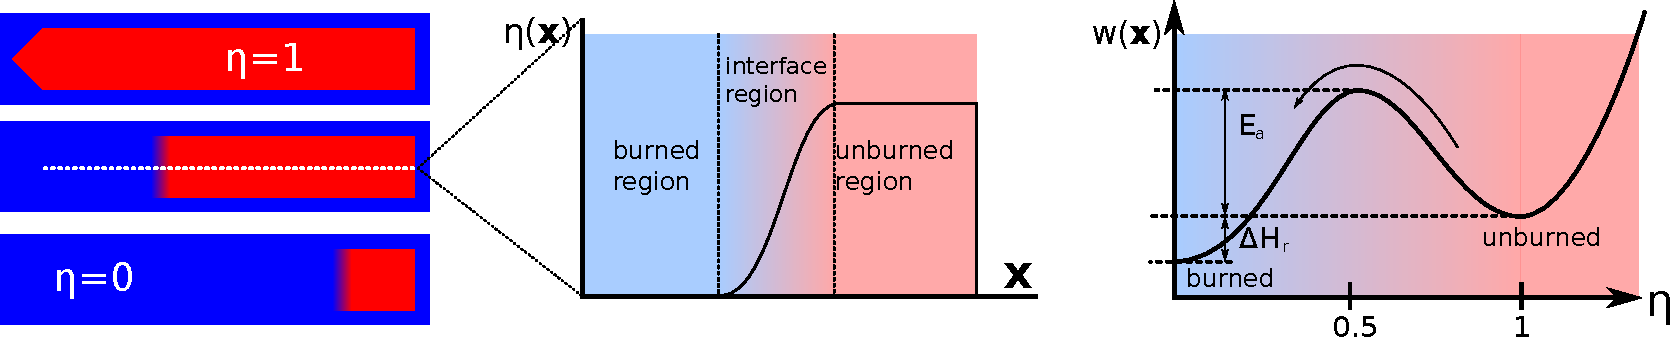
\includegraphics[width=\linewidth]{figures/u_vs_eta.pdf}
  \caption{%
    The order parameter $\eta$ representations---(a) Order parameter $\eta=1$ shows burned region, $\eta=0$ shows the unburned region and the interface region is $0 < \eta < 1$, (b) The representation of order parameter $\eta$ in terms of burned, unburned and interface regions along the length of the coupon, (c) The representation of free energy $w(\eta)$ in terms of  burned, unburned and interface regions 
  }
  \label{fig:burn}
\end{figure}

The order parameter functions simultaneously a thermodynamic reaction coordinate and an indicator function describing the geometry of the unburned region.
Here and subsequently, we denote the domain of interest as $\Omega\subset\mathbb{R}^n$.
We now begin our construction of a phase field model through the establishment of a free energy functional $f:C_2(\Omega,[0,1])\to\mathbb{R}$, given by,
\begin{equation} \label{eq:freeenergy}
  f[\eta]=\int_{\Omega} \Big[ \lambda w(\eta)+\frac{1}{2}\varepsilon^2\kappa{\left| {\nabla}{\eta} \right|}^2\Big]\,\diff\bm{x}, 
\end{equation}
where square brackets should be understood to indicate dependencies on the enclosed arguments and their spatial\slash temporal derivatives.
Normal invariant notation ($\nabla$ indicates the gradient, $\Delta$ the Laplacian, etc.) is employed.
The first term in the integrand indicates the chemical potential, $w$, which is generally a differentiable multiwell function with minima at $0$ and $1$ (\cref{fig:burn}).
The coefficient $\lambda$ is, for practical purposes, a scaling factor, but also admits interpretation as a Lagrange multiplier that may be scaled arbitrarily to bring the solution close to the sharp interface limit.
The second term in the integrand introduces nonlocality by penalizing gradients in $\eta$.
The coefficient $\kappa$ can be interpreted as the energy of the interface (i.e., surface tension) between the burned and unburned region; here, we simply view it as a numerical regularization.
The parameter $\varepsilon$, then, is a parameter that controls the length scale of the solution, and will be discussed in more detail subsequently.

The free energy functional $f$ provides the basis for the construction of a kinetic evolution equation. 
Adopting the classical {\it ansatz}, following non-equilibrium thermodynamic theory as well as the classical Ginzburg-Landau theory \cite {landau1950theory} that the order parameter evolves proportionally to the gradient of the free energy, i.e., following the $L_2$ gradient flow.
A kinetic variable, called the ``mobility'' $(L)$ is used scale the flow of $\eta$.
As will be shown subsequently, dividing by the length scale $\varepsilon$ is necessary to prevent dependence of the flame speed on the numerical burn width.
The equation governing the evolution is given by the following:
\begin{align}
  \frac{\partial\eta}{\partial t}
  =-\frac{L}{\varepsilon} \frac{\delta f}{\delta \eta}
  - L \left[\frac{\lambda}{\varepsilon}\frac{\partial w}{\partial \eta}-\varepsilon\kappa \Delta\eta \right].\label{eq:governing}
\end{align}
where $\delta/\delta\eta$ is the variational derivative.
The relatively low order of \cref{eq:governing} makes it readily solvable using optimized explicit methods, as discussed in \cref{Computation}.
Coupling to additional physics occurs through the modification of \cref{eq:freeenergy} to include other thermodynamic contributions such as thermal or elastic free energies, which are then integrated into the governing equation through the variational derivative.
As we will show, however, the reactive and diffusive components alone suffice to capture a broad range of SCP behavior.

\subsection{Determining burn rate in the limit}

Of particular interest in this present work is the connection of the governing equation to the burn rate in the sharp-interface limit.
To begin, we derive the relationship between one-dimensional burn rate and model parameters in a single-species material, in order to interpret the model parameters ($L,\varepsilon$, etc) in terms of measurable properties.
For the case of steady burning, we approximate
\begin{align}
  \eta_\varepsilon(x,t) &= f(\xi)  &   \xi = \frac{x-ct}{\varepsilon},
\end{align}
where $f$ is a $C_2$ function satisfying: (1) $f(\xi)=0$, $f'(\xi)=0$, and $\xi\le-\varepsilon/2$; (2) $f(\xi)=1$, $f'(\xi)=0$, and $\xi\ge\varepsilon/2$; (3) antisymmetry of $f(\xi)- \frac{1}{2}$ about $\xi=0$.
We do not currently specify any limits on $\varepsilon$, but will show that the solution satisfies the governing equations and scales with $\varepsilon$.
Now, substituting into the governing equation produces
\begin{align}
  -\frac{c}{\varepsilon}\frac{\diff f}{\diff \xi} = -L\Big[\frac{\lambda}{\varepsilon}\frac{\diff w}{\diff f} - \frac{\kappa}{\varepsilon}\frac{\diff^2f}{\diff x^2}\Big].\label{eq:subswithf}
\end{align}
The nonlinearity induced by the chemical potential renders \cref{eq:subswithf} unsolvable in the general case, which is undesirable as we seek a general relationship between the chemical potential, mobility, and burn width.
Therefore we seek a solution in the weak form by integrating both sides over the region $[-\varepsilon/2,\varepsilon/2]$:
\begin{align}
  c\int_{-\varepsilon/2}^{\varepsilon/2}\frac{\diff f}{\diff \xi}\,\diff \xi + L\kappa\int_{-\varepsilon/2}^{\varepsilon/2}\frac{\diff^2f}{\diff x^2}\,\diff \xi = L\int_{-\varepsilon/2}^{\varepsilon/2}\frac{\diff w}{\diff f}\,\diff \xi.
\end{align}
By inspection, and application of the properties of $f$, we find that the first integral reduces to unity, and the second to zero.
Next, applying a change of basis, the integral on the right-hand side becomes
\begin{align}
  \int_0^1\frac{\diff w}{\diff f}\frac{\diff \xi}{\diff f}\diff f.\label{eq:dwdfdxidf}
\end{align}
From this we derive the first important result, that flame speed $c$ does not depend on the barrier height (activation energy) of $w$.
The proof of this follows by noting that $w$ can be additively decomposed into two functions that are symmetric and antisymmetric about $f=0.5$; $w(f) = w_s(f) + w_a(f)$. 
Because barrier height will contribute to $w_s$, but not to $w_a$, it then follows that $dw_s/df$ is antisymmetric about $f=0.5$.
Recalling that $f-0.5$ is antisymmetric about $f=0.5$, we see that $d\xi/df$ is symmetric, and consequently
\begin{align}
  \int_0^1\frac{\diff w_s}{\diff f}\frac{\diff \xi}{\diff f}\,\diff \xi = 0,
\end{align}
concluding the proof of the above result.
Since the speed depends on the antisymmetric part of the chemical potential only, we can re-write it in terms of a template function $\hat{w}_a$ where $\hat{w}_a(0)=0, \hat{w}_a(1)=1$ so that 
\begin{align}
  w = w_0 + (w_1-w_0)\hat{w}_a + w_{1/2}w_s
\end{align}
where $w_0$ and $w_1$ are parameters that can be calibrated for the material.
This leads finally to the relation
\begin{align}\label{eq:c_to_L}
  c = \lambda L(w_1-w_0)\gamma[\hat{w}_a],
\end{align}
where $\gamma$ is a constant determined by evaluating \cref{eq:dwdfdxidf} for the choice of template function.
From this we see that, in the one-dimensional case, the mobility is proportional to the regression rate divided by the energy difference associated with the reaction.
As $\varepsilon\to0$, we obtain the sharp interface limit, for which the above analysis shows the one-dimensional case to be unchanged.
As the diffuse thickness goes to zero, the interface at any point can be approximated as planar (due to the $C_2$ restriction on $\eta$) within a sufficiently small neighborhood, allowing the interface motion at all points to be regarded locally as one-dimensional.
Therefore, we conclude that \cref{eq:c_to_L} holds as a general statement of the relation between speed and mobility in the sharp-interface limit.

\subsection{Chemical potential specialization}

We showed in the previous section that the behavior of the model is insensitive to the precise choice of chemical potential $w$ (up to scaling), and is in fact impervious to the magnitude of the energy barrier.
Therefore we adopt, for convenience, a polynomial approximation to $w$:
\begin{equation} \label{eq:11}
  w(\mathbf{x},\eta) = \sum_{i=1}^N a_{n}(\mathbf{x})\,\eta^n(\bm{x}),
\end{equation}  
where $N=4$ but can be increased if greater complexity is needed.
Re-writing the polynomial in order to satisfy the conditions of stability at $0,1$ and prescribed values $w_0,w_{1/2},w_{1}$ at $0,1/2,2$, respectively, the equations
\begin{align} \label{eq:12}
  w(0) &= w_0
  &
    \frac{\partial w}{\partial\eta}\Big|_{\eta=0} &= 0
  &  w_{1/2} &= w(1/2) 
  &
    w(1)   &=   w_1
  &
    \frac{\partial w}{\partial\eta}\Big|_{\eta=1} &= 0,
\end{align}
produce the polynomial coefficients
\renewcommand{\arraystretch}{0.6}
\begin{align} \label{eq:13}
  \begin{bmatrix}
    a_0 \\ a_1 \\ a_2 \\ a_3 \\ a_4 
  \end{bmatrix}
  = 
  \begin{bmatrix}
    1 & 0 & 0 \\
    0 & 0 & 0 \\
    -11 & 16 & -5 \\
    18 & -32 & 14 \\
    -8 & 16 & -8 \\
  \end{bmatrix}
  \begin{bmatrix}
    w_0 \\ w_{1/2} \\ w_{1} 
  \end{bmatrix}.
\end{align}
It is possible to tailor $w$ to a form that is informed by the chemistry, in which the form of $w$ corresponds to the reaction energy as a function of reaction coordinate $\eta$.
It is also possible to extend this potential to capture multi-phase (solid\slash liquid\slash gas) behavior through the addition of another minima at a value of $\eta$ designated to be a liquid phase.
In this work, the aim is to show the efficacy of a simple model in capturing regression rates; these extensions will be considered in future work.

\subsection{Multi-species interactions}

In composite propellants, multiple constituent species interact chemically to sustain deflagration in the thermodynamic regime of interest.
Some oxidizers (such as AP) will burn independently as monopropellants, whereas fuel binders (HTPB\slash PBAN) decompose but do not burn on their own \cite{ye2013analysis}.
Therefore a regression rate model must capture the effect of the species concentration and spatial distribution on regression rate.
We introduce a spatial variable, called the diffuse species field ($\phi(\bm{x})$) to determine pointwise concentration of oxidizer and binder.
We adopt the convention that $\phi=1$ corresponds to pure oxidizer, $\phi=0$ to pure binder.


\begin{figure}
  \centering
  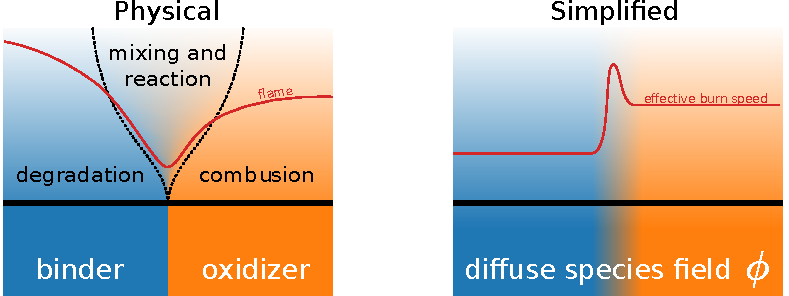
\includegraphics[height=4cm]{figures/mix.pdf}
  \caption{
    Schematic illustrating the concept of the diffuse species concentration simplification.
    (Left: Physical) At the boundary, binder and oxidizer diffuse and mix at the species boundary, which enables combustion to occur.
    Far from the boundary, the binder degrades and the oxidizer burns, and the result is a flame that is close to the solid interface near the species boundary, but further away from the oxidizer interface and even further from the binder interface.
    Physically this produces differing regression rates in the three regimes of interest.
    (Right: Simplified) The diffuse species field $\phi$ is used to adjust the effective regression rate depending on the species---generally, slow in the binder, faster for the oxidizer, and fastest in the interfacial region.
  }
  \label{fig:mix}
\end{figure}

Material characteristics can then be represented simply using a mixture rule: for some property $\pi$, the effective property is given by $\pi_\mathrm{eff}=\pi_\mathrm{binder}(1-\phi) + \pi_\mathrm{oxidizer}\phi$. 
We aim to use continuous material variability to capture the effect of material heterogeneity on regression rate.
Physically, this is a consequence of the mass fluxes causing mixing and facilitating chemistry, which results in fast\slash slow reaction rates and, consequently, differing heat fluxes into the solid.
Far from the binder\slash AP boundary, the AP can support a self deflagration flame, which ensures that there is some heat transfer from the flame back to the solid---driving the surface regression.
Also far from the interface, but over the binder, any heat fed back to the solid goes to transforming the species and the phase to gaseous fuel species.
This is an endothermic process and results in a generally slow binder surface regression.
Near the interface, the gaseous fuel and oxidizers have strong gradients and as a consequence diffuse rapidly towards each other.
Where they meet in stoichiometric proportions there is a diffusion flame---at least away from the solid surface, where the heat transfer is to fast back to the solid and temperatures too low for combustion.
This resulting slightly lifted diffusion flame, and lean\slash rich premixed flames that sit at the base of the diffusion flame, cause very steep temperature gradients.
Since this causes very high heat transfer from the flame to the solid, near the interface, the local regression rate is considerably higher near the solid\slash solid interface.

To capture this phenomenon, it is necessary to modify the property field in such a way as to capture local interface-specific properties; specifically, burn rate is
\begin{align}
  \pi_\mathrm{eff}=\pi_{\mathrm{binder}}(1-\phi) + \pi_{\mathrm{oxidizer}}\phi + 4\,\phi\,(1-\phi) \pi_{\mathrm{interface}}
\end{align}
where $\pi_{\mathrm{interface}}$ is an interface correction term, and $\pi\to L$, the mobility, which is linearly proportional to the burn rate, and affects only the region within the diffuse solid\slash solid boundary.
In this way, we capture the effect of interface mixing and reaction chemistry (\cref{fig:mix} left) using a reduced order surrogate model for pressure-informed burn speed (\cref{fig:mix} right), without incurring the cost of a full gas-phase simulation.

\section{Computation}  \label{Computation} 

\begin{figure}
  \centering
  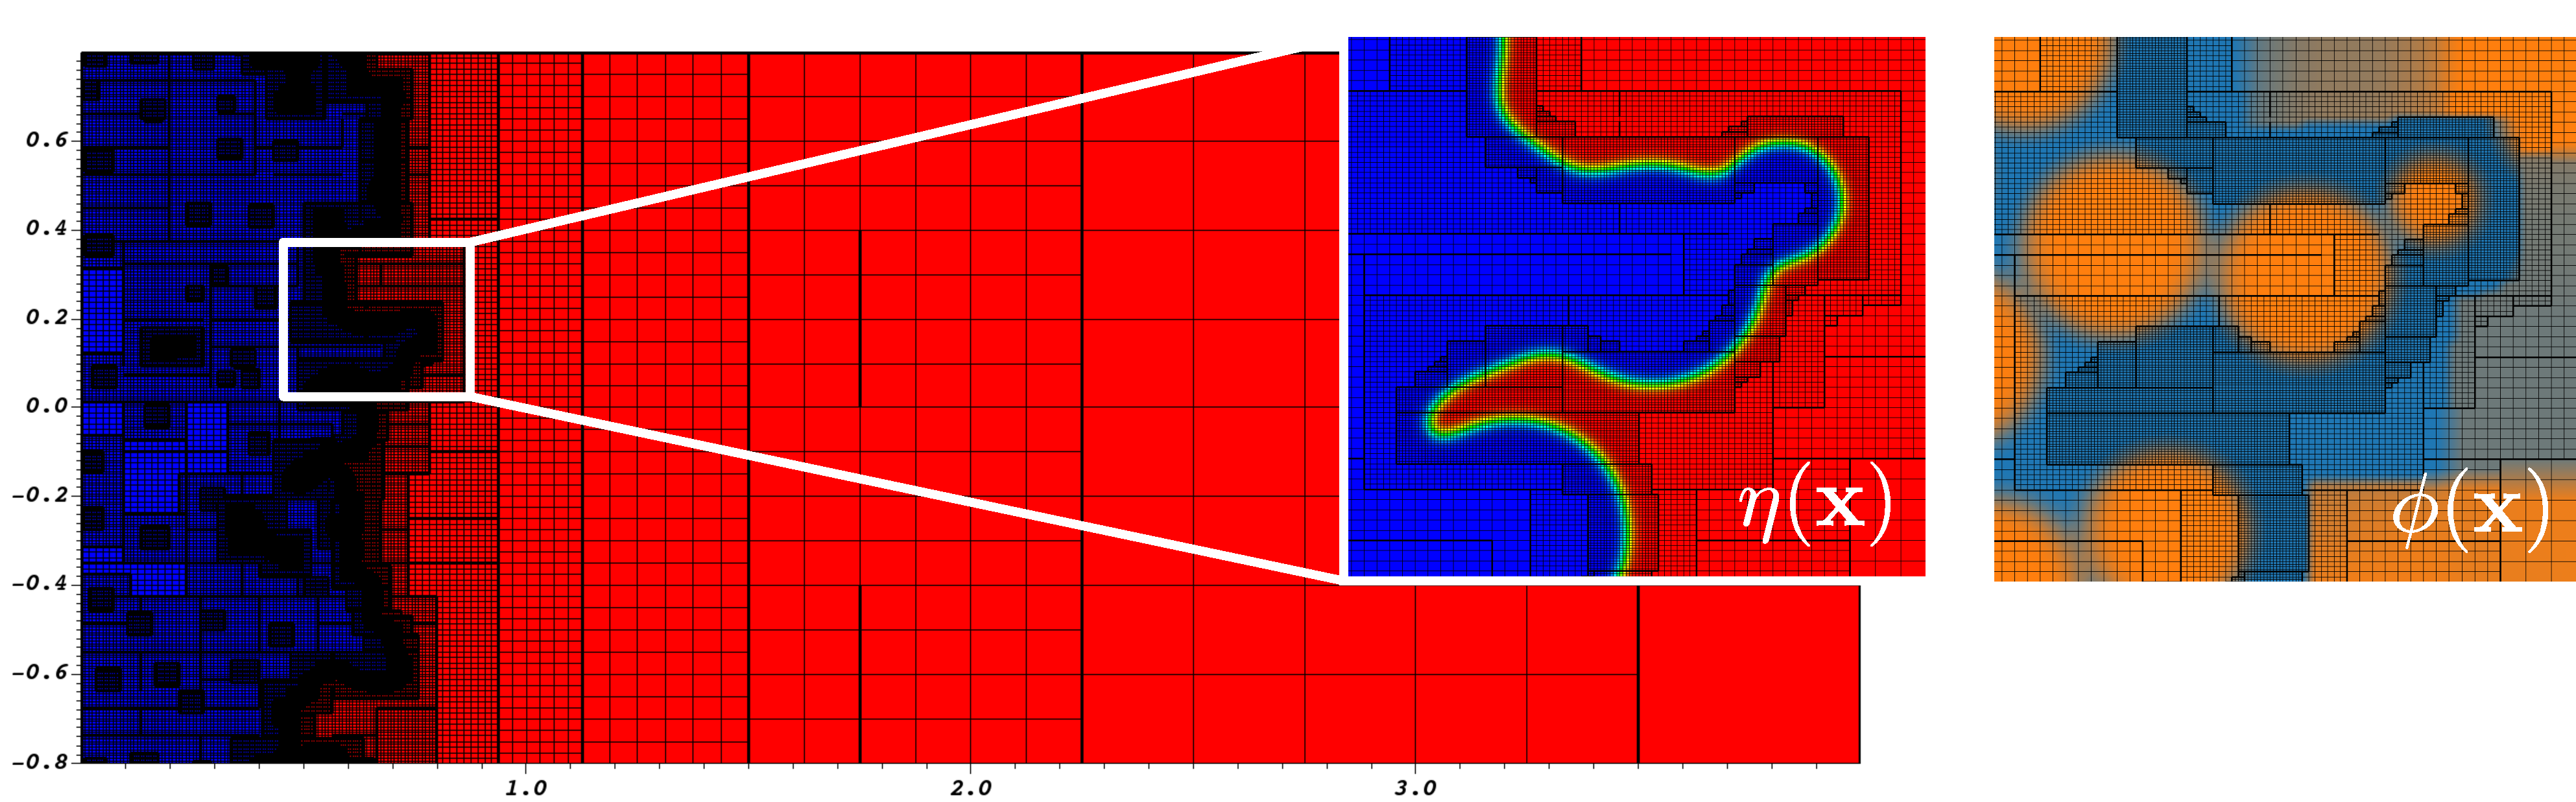
\includegraphics[width=\linewidth]{figures/amr.pdf}
  \caption{
    Sample result (from packed spheres case) illustrating the use of block-structured adaptive mesh refinement at the boundary.
    The base level grid is very coarse (left).
    Multiple BSAMR levels allows for refinement at the $\eta$ boundary (left popout).
    Refinement is based only on $\eta$ (not on $\phi$), and $\phi$ is updated only on an as-needed basis to enhance performance (right popout).
  }
  \label{fig:amr}
\end{figure}

One of the primary limitations of diffuse interface methods is the computational cost.
By definition, there is a distinct scale separation between the application scale and the diffuse interface scale; indeed, if the scales are not properly separated, the model is unlikely to be accurate.
Computationally this presents a challenge, as full resolution of the entire domain is both prohibitively expensive and unnecessary.
Adaptive mesh refinement (AMR) is a computational strategy for diffuse interface methods by selectively refining at the diffuse interface and coarsening elsewhere as appropriate.
Block-structured AMR (BSAMR) is a particularly attractive type of AMR (\cref{fig:amr}).
The BSAMR strategy is to divide the domain into distinct levels, each corresponding to a level of refinement, and then facilitates communication between levels through averaging and interpolation between timesteps.
This data structure is particularly advantageous for performance, as the individual patches can easily be distributed across a distributed memory computational platform.
BSAMR also allows for temporal subcycling, automatically reducing the timestep and increasing the number of iterations on finer levels.
This eliminates common CFL difficulties in explicit methods that can arise during mesh refinement.

In this work, we use an in-house code ``Alamo'' to implement and test the diffuse interface model \cite{runnels2021massively}.
Alamo is built on the AMReX library \cite{zhang2019amrex}, and implements a variety of physical models ranging from fluid mechanics to microstructure evolution.
A forward Euler temporal scheme is used to evolve the kinetic equation with finite difference spatial derivatives.
The coarse level timestep is st to $2.5\times10^{-5}$ seconds, and a temporal substep factor of 2 is used between refinement levels, for a finest-level timestep of approximately $2\times10^{-8}$ seconds.
Regridding is set to occur every 100 timesteps (on the coarse level) and occurs whenever the following condition holds:
\begin{align}
  |\nabla \eta|\,|\Delta \bm{x}| \ge 0.01,
\end{align}
where $\Delta\bm{x}$ is the vector of grid spacings (\cref{fig:amr} left popout).
Refinement does not currently occur at solid/solid boundaries, unless they intersect the burn interface, in order to maximize performance.
Moreover, initiation of $\phi$ occurs on the finest level only, due to the potential cost in calculating the value of $\phi$.
Note that because coarse values of $\phi$ are calculated before refinement, but averaged after refinement, this produces a distinction between pre-burn and post-burn plots of $\phi$ (\cref{fig:amr} right popout).
Because the solution is insensitive to this approximation, it is possible to simulate arbitrarily complex composite geometries with no additional computational cost.

\section{Results} \label{Results} 


\begin{table} 
  \centering
  \begin{tabularx}{\linewidth}{llXXXXX} 
    \toprule
    \bf Parameter name & \bf Symbol & \bf AP & \bf PBAN & \bf HTPB & \bf AP+ & \bf AP+\\
    \bf                & \bf        & \bf    & \bf      & \bf      & \bf PBAN & \bf HTPB\\
    \midrule
    Flame speed exponent (-)      & $n_\mathrm{AP}$ &  1.042 & 0.0 & 0.0 & 0.0 & 0.0\\ 
    Flame speed coefficient (mm/s)& $r_\mathrm{AP}$ &  1.222 & 0.1 & 0.5 & 10.01 & 12.5 \\
    Base pressure (MPa)           & $p_\mathrm{p}$   &  1.0 \\ 
    Burned energy (MPa)           & $w_0$   & $0.0$\\
    Unburned energy (MPa)         & $w_1$   & $1.0$ \\
    Activation energy (MPa)       & $w_{1/2}$ & $2.0$ \\
    Diffuse width (mm)            & $\varepsilon$ & 0.0005 \\
    Chemical potential factor (-) & $\lambda$ & 0.001 \\
    Interface energy (MPa)        & $\kappa$ & 1.0 \\
    Shape constant (-)            & $\gamma$ & 0.02726\\
    \bottomrule
  \end{tabularx}
  \caption{AP, PBAN, HTPB parameters for the solid phase model}
  \label{tab:parameters} 
\end{table}


In this section, we apply the computational phase field model to study a variety of SCP configurations, with the aim of establishing its validity and predictive ability.
In this study, we use AP for the oxidizer and consider binders of both PBAN and HTPB.
Four different cases are considered: the coupon of pure AP (pure AP); a thin layer of PBAN sandwiched between AP (AP\slash PBAN sandwich); a thin layer of HTPB sandwiched in between AP (AP\slash HTPB sandwich); and AP sphere particles with HTPB binder (AP\slash HTPB packed spheres).

\subsection{Pure ammonium perchlorate burning}

We begin with a calibration of the model for the pure AP case to established, experimentally measured pressure-dependent AP regression rates.
The pressure-dependent mobility is calculated using \cref{eq:c_to_L}, and is reported in \cref{tab:parameters} along with parameters used in this work.
A simulation domain of $4\,\mathrm{mm} \times 0.5\,\mathrm{mm}$ was used with a base mesh of $16 times 2$ cells and 7 levels of BSAMR refinement.
Burn rates are calculated and compared to legacy experimental data reported in \cite{price1983combustion}.
To achieve consistency with experimental measurements, such as those reported in \cite{price1984combustion, knott2002modeling, hayakawa2000effect} which use a break-wire method to measure burn speed, we measure the instantaneous effective position of the interface as the location of the leading point of the burn front.

Close agreement to experimental values are recovered (Reported in \cref{fig:sandwich_ap_pban_fs_vs_pressure,fig:sandwich_AP_HTPB_plot}).
This is unsurprising, given the analytic relation between mobility, chemical potential, and burn rate; nevertheless, it indicates that the model will produce realistic results for this type of monopropellant burn.

\subsection{AP and PBAN sandwich}

\begin{figure}
  \centering
  \begin{subfigure}{0.48\linewidth}
    \includegraphics[height=5cm]{results/AP_HTPB_Sandwich/layout.pdf}
    \caption{Dimensions of sandwich structure consisting of AP ({\color{C1}gold}) and HTPB or PBAN binder layer ({\color{C0}blue}).}
    \label{fig:sandwich_layout}
  \end{subfigure}\hfill
  \begin{subfigure}{0.48\linewidth}
    \includegraphics[height=5cm]{results/AP_PBAN_Sandwich/fs_vs_pressure.pdf}
    \caption{Comparison of model results for flame speed in pure AP and AP+PBAN sandwich structure } 
    \label{fig:sandwich_ap_pban_fs_vs_pressure} 
  \end{subfigure}
  \caption{
    AP/PBAN sandwich burn results
  }
\end{figure}


In realistic SCPs, the behavior induced by the SCP geometry (complex interface surface of binder with the AP packed AP particles) results in complex burn behavior that eludes simplistic analysis.
Therefore, to better understand the interactions between oxidizer and binder, sandwich structures provide a simplified yet nontrivial case study.
Sandwich structures have been examined in a variety of experimental reports, such as studied with and without catalysts and the influence of the liquid phase \cite{ermolaev1970laws,chorpening2002emission,chakravarthy2003plateau,chakravarthy2004intermittent, ishitha2014studies,gnanaprakash2017combustion,gnanaprakash2019effect}, over the span of the past several decades.
The geometry of sandwich structures is simple: a laminate of binder between two blocks of AP (\cref{fig:sandwich_layout}).
Here, a $4\,\mathrm{mm} \times 0.5\,\mathrm{mm}$ geometry was used with a laminate thickness of 0.1\,mm.
As with the pure AP case, a $16 \times 2$ base grid was used with 7 levels of mesh refinement, and a diffuse interface thickness of $\zeta=0.015$ was used.
Pressures ranging from 500\,kPa to 4\,MPa were considered, and parameters were adjusted by comparison to the values reported by Price {\it et al.} \cite{price1983combustion}.

In this simulation the parameters for AP were help constant with the values that were found for the pure AP combustion and we calibrated the binder parameters only, which are reported in \cref{tab:parameters}.
The resulting burn rate calculations show a very close match between the model and experimentally reported values (\cref{fig:sandwich_ap_pban_fs_vs_pressure}).
An interesting point to note is that, although a pressure power law form had been assumed for both the PBAN and mixture regions, the best exponential coefficient was found to be zero, i.e., constant value was determined to best match the experiments.

A key feature of this model is its ability to capture the complex regression morphology in addition to the regression rate.
A comparison was made between experimentally observed burn front shapes (\cref{fig:sandwich_shape}) and numerical simulation (\cref{fig:sandwich_ap_pban_traces}).
For the numerical results, traces are plotted at every 10\,ms; blue traces every 100\,ms.

The simulated burn behavior, qualitatively, exhibits a high degree of similarity to that observed in experiment.
At low pressures, AP burns very slowly because the pressure is too low to maintain monopropellant burning.
This manifests as a deep grooved burn profile, caused by the differential between the burn speeds in the interface region and the pure AP region.
Remarkably, we even observe the slight dimple present in the binder layer, which is the result of an excess of binder beyond that which is needed to react locally with AP near the interface.
At high pressure, where AP is able to effectively self-react, an opposite trend is observed: the AP burns faster than the binder, leaving a distinctive protrusion of the binder.

\begin{figure}
  \begin{subfigure}{0.48\linewidth}\centering
    \includegraphics[height=6cm]{results/AP_PBAN_Sandwich/price1983combustion_figure1.png}
    \caption{ Experimental observations of burn profiles for low pressure (a,d), medium pressure (b,e), and high pressure (e,f); reproduced from Price {\it et al.} \cite[Fig 1]{price1983combustion}}
    \label{fig:sandwich_shape}
  \end{subfigure}\hfill
  \begin{subfigure}{0.48\linewidth}\centering
    \includegraphics[height=6cm]{results/AP_PBAN_Sandwich/traces_P=0.5.pdf}%
    \includegraphics[height=6cm]{results/AP_PBAN_Sandwich/traces_P=0.8.pdf}%
    \includegraphics[height=6cm]{results/AP_PBAN_Sandwich/traces_P=2.0.pdf}%
    \includegraphics[height=6cm]{results/AP_PBAN_Sandwich/traces_P=4.0.pdf}
    \caption{Traces of the burn front evolving over time. Blue traces are plotted at time intervals of $\Delta t = 100\,\mathrm{ms}$. From left to right the pressures are 0.5, 0.8, 2, and 4\,MPa.}
    \label{fig:sandwich_ap_pban_traces}
  \end{subfigure}
  \caption{AP/PBAN Sandwich: comparison between experimentally observed and numerically predicted interface morphology}
\end{figure}

\subsection{AP and HTPB sandwich}


The setup for a sandwich structure composed of AP with an HTPB binder is identical to the AP\slash PBAN case except for the selection of parameters for the binder and binder interaction.
Importantly, again, the AP parameters are unchanged.
Experimental data from Knott {\it et al.} \cite{knott2002modeling} is used for calibration of the binder parameters.
It should be noted that we include the experimental data for all binder thickness for comparison from this work, observing that the difference between them is relatively small.

Parameters for HTPB were determined by grid search.
As with the PBAN case, it was determined that the pressure law exponent was negligibly small, meaning that a constant value for the burn rate sufficed to produce the observed results.
Comparison to experimental data indicates a very close match between the simulated regression rate and the observed rate (\cref{fig:sandwich_AP_HTPB_plot}).
It is of interest that an inflection in the burn rate is observed at approximately 8\,kPa, matching a similar trend in the experiment.
Despite the similar mathematical form to the AP\slash PBAN case, this demonstrates that nonlinear phenomena can be captured with this model.
In this case, we attribute this change to the more extreme morphology in the interface.

The burn profile is qualitatively similar to that calculated for AP and PBAN (\cref{fig:sandwich AP/HTPB propagation}).
In both cases, the interface regresses most quickly at the solid\slash solid interface, due to the enhanced burn chemistry enabled by the mixing of the binder and AP mass fluxes.
As the pressure is increased, the AP matrix is able to sustain a reaction independently.
At high enough pressure, the pure AP regression rate exceeds that of the solid\slash solids interface, essentially leaving a flat AP surface.
In all cases, a protrusion formed by the HTPB binder is left behind. 
At low pressure the binder is quickly consumed, but at high pressure it is persistent.
We note that such a protrusion would, in reality, be unstable and unlikely to remain attached as indicated by the model.
We expect, however, that the quantity of HTPB not effectively burned would likely correspond to the volume left behind in this model.

\begin{figure}
  \begin{subfigure}{0.55\linewidth}
    \includegraphics[height=6cm]{results/AP_HTPB_Sandwich/fs_vs_pressure.pdf}
    \caption{Comparison of model results for flame speed in pure AP and AP+HTPB sandwich structure.}
    \label{fig:sandwich_AP_HTPB_plot}
  \end{subfigure}\hfill%
  \begin{subfigure}{0.4\linewidth}
    \includegraphics[height=6cm]{results/AP_HTPB_Sandwich/traces_P=0.2.pdf}%
    \includegraphics[height=6cm]{results/AP_HTPB_Sandwich/traces_P=0.8.pdf}%
    \includegraphics[height=6cm]{results/AP_HTPB_Sandwich/traces_P=2.0.pdf}%
    \includegraphics[height=6cm]{results/AP_HTPB_Sandwich/traces_P=4.0.pdf}
    \caption{Traces of the burn front evolving over time. Blue traces are plotted at time intervals of $\Delta t = 100\,\mathrm{ms}$. From left to right the pressures are 0.5, 0.8, 2, and 4\,MPa.}
    \label{fig:sandwich AP/HTPB propagation}
  \end{subfigure}
  \caption{Regression rates in AP/HTPB sandwich structures with varying pressure}
\end{figure}

\subsection{Packed AP spheres in HTPB matrix}

In this section we test the predictive capability of the model by considering the practical case of packed AP spheres (with two different mass concentrations) embedded in an HTPB matrix.
The initial geometry of the oxidizer particles are modeled as spheres similar to previous studies (\cref{fig:packedspheres_layout}). 
This test case is representative of practical SCP, and we emphasize that the model parameters are not adjusted to match the results to experimental values; the same parameters determined in the previous sections are used, and the only change in this work is the geometry of the binder and matrix.


The 2D simulation domain is specified to be $4\,\mathrm{mm} \times 1.6\,\mathrm{mm}$.
Mass fractions of $78\%$ and $64\%$ AP are considered, which corresponds to volume fractions of $62\%$ and $45\%$, respectively.
Although AP particles are generally irregular, we follow precedent \cite{dennis2019combustion} in the use of non-overlapping spheres for this calculation.
(We note that the effect of non-spherical particles is non-trivial, and will constitute future work.)
The domain is filled with a unimodal distribution of spheres corresponding to the aforementioned volume fractions.
In order to faithfully represent the 3D sample with a 2D model, a 3D domain is packed with spheres using the Jodrey and Tory algorithm \cite{jodrey1985computer} implemented in OpenMC \cite{romano2015openmc}.
A slice of the 3D spheres in the domain is then used to generate the effective unimodal distribution in 2D.
To generate the diffuse species field corresponding for the packed spheres, the formula is used
\begin{align}
  \phi(\bm{x}) = 1 - \prod_{n=1}^N\Bigg(\frac{1}{2} + \frac{1}{2}\operatorname{erf}\Big((|\bm{x}-\bm{x}_n| - r_n)/\zeta\Big)\Bigg)
\end{align}
where $\zeta$ determines the diffusivity of the solid\slash solid interface ($\zeta\to0$ recovers the sharp interface limit) and was determined here to be $\zeta=10\,\mu\mathrm{m}$.
($\phi(\bm{x})$ for the packed spheres is plotted in the right pop-out of \cref{fig:amr}.)

\begin{figure}
  \centering
  \begin{subfigure}{0.5\linewidth}\centering
    \includegraphics[height=5cm]{results/AP_HTPB_PackedSpheres/layout.pdf}\hfill
    \caption{}
    \label{fig:packedspheres_layout}
  \end{subfigure}%
  \begin{subfigure}{0.5\linewidth}\centering
    \includegraphics[height=5cm]{results/AP_HTPB_PackedSpheres/fs_vs_pressure_kohga.pdf}
    \caption{}
    \label{fig:packedspheres_fs_vs_pressure}
  \end{subfigure}
  \caption{
    Results for packed AP spheres in an HTPB matrix.
    (a) Visualization showing the generated 3D packing and the corresponding 2D slice.
    (b) Results for the model with mass fractions of $78\%$ and $64\%$, compared to experimental data reported in \cite{kohga2011burning}.}
\end{figure}

The burn rate is determined as before by fitting the slope of the effective interface position using linear regression. 
Unlike with the pure AP or sandwich cases, a substantial amount of variability is observed in the leading point burn location.
This is due to the high degree of complexity observed in the burn front, which will be discussed shortly.
To represent this high degree of variability, the approximate variance is calculated as the RMS difference between the instantaneous velocity (calculated by finite difference between timesteps) and the approximate velocity, and represented using error bars.

Simulations were conducted for pressure from 1--7\,MPa at 1\,MPa intervals for both volume fractions, and compared to corresponding experimental observations for equivalent SCPs as reported by Kohga \cite{kohga2011burning} (\cref{fig:packedspheres_fs_vs_pressure}).
A close match is observed, particularly for the $64\%$ AP case.
A reasonably close match is also observed for the $78\%$ AP case (particularly at $p=6\,\mathrm{MPa}$), although we do note a deviation in the slope.
Given the lack of error reporting in the original source, it is impossible to conclusively determine the severity of the deviation; we do, however, note that there is a substantial amount of variance between this and other experimental reports, and so we conclude that the model's deviation is reasonable.

Qualitatively, the results demonstrate marked dependence both on pressure and on concentration, which is well-known to exist.
This shows that the approximations made in the model, despite their simplification of complex burn behavior, do not introduce substantial error.
It also shows the predictive power of the model, which is especially apparent here, since the parameters were unchanged from the values obtained in the sandwich calibration tests.
(Obviously, a much closer match could be attained if the parameters had been calibrated for this case!)
We suggest, therefore, that this model can be used in its present form to investigate the behavior of other types of SCP configurations with reasonable accuracy.


\begin{figure}
  \begin{subfigure}{0.25\linewidth}
    \includegraphics[height=8cm]{results/AP_HTPB_PackedSpheres/output_8795000/traces.png}%
    \caption{$\mathrm{MF}=64\%,p=1\,\mathrm{MPa}$}\label{fig:Packed_low_low}
  \end{subfigure}%
  \begin{subfigure}{0.25\linewidth}
    \includegraphics[height=8cm]{results/AP_HTPB_PackedSpheres/output_8795091/traces.png}%
    \caption{$\mathrm{MF}=78\%,p=1\,\mathrm{MPa}$}\label{fig:Packed_high_low}
  \end{subfigure}%
  \begin{subfigure}{0.25\linewidth}
    \includegraphics[height=8cm]{results/AP_HTPB_PackedSpheres/output_8795042/traces.png}%
    \caption{$\mathrm{MF}=64\%,p=4\,\mathrm{MPa}$}\label{fig:Packed_low_high}
  \end{subfigure}%
  \begin{subfigure}{0.25\linewidth}
    \includegraphics[height=8cm]{results/AP_HTPB_PackedSpheres/output_8795588/traces.png}%
    \caption{$\mathrm{MF}=78\%,p=4\,\mathrm{MPa}$}\label{fig:Packed_high_high}
  \end{subfigure}
  \caption{
    Traces illustrating observed burn front behavior for varying mass fractions and pressures.
    Gray traces are plotted at intervals of 50\,ms, blue traces at intervals of 250\,ms.
  }
  \label{fig:packedspheres_traces}
\end{figure}


As with the sandwich cases, we also investigate the morphological details of the solid phase regression.
Unlike with the previous cases, in which the front approaches a steady-state shape, the randomness of the the sphere packing induces a highly random and richly complex burn front. 
Here, we present trace plots illustrating the progression of the burn front in time (\cref{fig:packedspheres_traces}).
The traces are superimposed on plots of the AP particle locations, and are plotted at 50\,ms intervals.
The trace diagrams illustrate the qualitative differences between the burn front surface time history.

At constant low pressure, we observe that the morphology of the low concentration AP (\cref{fig:Packed_low_low}) is substantially more complex than the high concentration (\cref{fig:Packed_high_low}).
This is unsurprising: low AP concentrations have lower interfacial surface area, and leave large islands of binder that have no AP with which to react.
On the other hand, high AP concentrations result in smaller and fewer binder islands, meaning that the majority of the binder is available to react with the AP and there is less waste.
A similar trend is observed at high pressure (\cref{fig:Packed_low_high,fig:Packed_high_high}).
Trends are also compared for both concentrations at 5\,MPa (\cref{fig:packed_single_front_track}); here it is clear that, aside from the obvious difference in flame speed, there is a distinct difference in morphology as well as the size and shape of left-behind islands.



\begin{figure}[t]
  \centering
  \begin{subfigure}{0.8\linewidth}\centering
    \includegraphics[height=0.2\linewidth,angle=-90]{results/AP_HTPB_PackedSpheres/output_8795043/combine_00000cell_thumbnail.png}%
    \includegraphics[height=0.2\linewidth,angle=-90]{results/AP_HTPB_PackedSpheres/output_8795043/combine_04000cell_thumbnail.png}%
    \includegraphics[height=0.2\linewidth,angle=-90]{results/AP_HTPB_PackedSpheres/output_8795043/combine_08000cell_thumbnail.png}%
    \includegraphics[height=0.2\linewidth,angle=-90]{results/AP_HTPB_PackedSpheres/output_8795043/combine_12000cell_thumbnail.png}%
    \includegraphics[height=0.2\linewidth,angle=-90]{results/AP_HTPB_PackedSpheres/output_8795043/combine_16000cell_thumbnail.png}
  \end{subfigure}
  \\
  \begin{subfigure}{0.8\linewidth}\centering
    \includegraphics[height=0.2\linewidth,angle=-90]{results/AP_HTPB_PackedSpheres/output_8795097/combine_00000cell_thumbnail.png}%
    \includegraphics[height=0.2\linewidth,angle=-90]{results/AP_HTPB_PackedSpheres/output_8795097/combine_04000cell_thumbnail.png}%
    \includegraphics[height=0.2\linewidth,angle=-90]{results/AP_HTPB_PackedSpheres/output_8795097/combine_08000cell_thumbnail.png}%
    \includegraphics[height=0.2\linewidth,angle=-90]{results/AP_HTPB_PackedSpheres/output_8795097/combine_12000cell_thumbnail.png}%
    \includegraphics[height=0.2\linewidth,angle=-90]{results/AP_HTPB_PackedSpheres/output_8795097/combine_16000cell_thumbnail.png}
  \end{subfigure}
  \caption{
    Comparison of burn profiles at $p=5\,\mathrm{MPa}$ for $64\%$ AP (left) and $78\%$ AP (right).
    Intervals are at $\Delta t = 0.16$\,s.
  }
  \label{fig:packed_single_front_track}
\end{figure}


\section{Conclusion}\label{Conclusion} 

In this work, we present a solid-phase model for calculating the burn rate and morphology for solid composite propellants using a diffuse interface method.
The model is based on classic work from phase field theory, which allows for the thermodynamics of the system to be captured faithfully in a geometrically arbitrary setting.
We demonstrate the interpretability between the model parameters and physical values, by showing the relationship between free energy, mobility, interface shape, and flame speed.
We then develop a scheme for reduced-order modeling of the effect of interface mixing on the burn rate, using a heuristic combustion model and diffuse species field parameter field.

The model is applied to a selection of experimentally verifiable SCPs.
It is first calibrated to AP monopropellant burn by comparison to legacy data.
Sandwich structures with both PBAN and HTPB binders are then used to calibrate the model parameters for a range of pressures.
Finally, the model is applied predictively (i.e., without adjusting parameters) to study packed AP spheres in an HTPB matrix at varying mass concentrations and varying pressures.
It is shown that the model matches experimental data very well, especially for the low concentration case.
The burn profiles are shown to match well with experimental observation, both for sandwich structures and packed spheres, demonstrating the model's ability to capture complex interface geometry.

An important conclusion that can be drawn from this work, regarding solid phase models of this type, is that it is necessary to explicitly account for interface content.
In other words, it is an oversimplification to simply rely on individual decomposition\slash burn rates; to do so will inevitably fail to capture the increased burn rate observed in SCPs burning below 1\,MPa.
It is also important to reiterate the connection between pressure, concentration, and islands of left-behind binder, which may have important implications for burn efficiency and production of waste binder.

We conclude this discussion with an overview of the many simplifications made in this work.
We have proposed a highly reduced-order model intended to capture the burn rate and morphology of SCPs, and we caution that care should be taken in the interpretation and extension of the model results.
The primary simplification is the approximation of the mobility, $L$ using a pressure and species dependent power law.
In reality, $L$ should be understood to depend primarily on temperature, which is determined by the heat flux, which is determined by the reaction chemistry, which is dependent on the mass flux, which in turn is dependent on the mobility.
We also note that all of the simulations considered here have been two-dimensional.
For the case of packed spheres, a three-dimensional study is likely needed to account for the effect of spheres (rather than apparent cylinders) in the SCP.
Investigation of these model extensions will be pursued in future work.

\section*{Acknowledgments}
BK and BR were supported by the Office of Naval Research [grant number \#N00014-21-1-2113].
MQ was supported in this effort by UCCS Department of Mechanical and Aerospace Engineering start-up funds.
This work used the Extreme Science and Engineering Discovery Environment (XSEDE) on the STAMPEDE2 supercomputer at the Texas Advanced Computing Center (TACC) through allocation TG-PHY130007; XSEDE is supported by the National Science Foundation [grant number ACI-1548562].
Finally, the authors gratefully acknowledge many discussions with Dr.~Brian Bojko that substantially strengthened this work.


\bibliographystyle{elsarticle-num}
\bibliography{library}



\appendix








\end{document}
